\documentclass[conference]{IEEEtran}
\usepackage{cite}
\usepackage{graphicx}
\usepackage{booktabs}
\usepackage{amsmath}
\usepackage{url}
\usepackage{xcolor}
\newcommand{\simval}[1]{\textcolor{red}{[#1]}}
\begin{document}

\title{Resource-Aware Deployment Scenarios for an AI-Driven Digital Twin in Predictive Maintenance}

\author{\IEEEauthorblockN{Muhammad Ayan Asif (22i-1097) and Ruhab Ahmad (23i-0559)}
\IEEEauthorblockA{FAST-NUCES, Islamabad, Pakistan}}

\maketitle

\begin{abstract}
This paper evaluates a reproducible Random Forest remaining-useful-life (RUL) baseline on NASA C-MAPSS FD001 and presents explicit cloud-only, edge-only, and hybrid deployment scenarios. The model uses causal 30-cycle windows and 66 features and is evaluated on the official 100-engine test set with three random seeds. Its measured mean RMSE is 15.0266 $\pm$ 0.5049 cycles and its mean MAE is 11.8558 $\pm$ 0.4167 cycles; these improve on the training-mean baseline by 65.1\% and 67.0\%, respectively. In the 61--90-cycle subgroup, however, the baseline's actual MAE is 8.12 cycles versus 21.96 for the RF across 15 engines. The placement comparison does not deploy services or transfer requests: it applies configured network and edge-compute assumptions to shared predictions and measured local timings. Therefore, its derived p95 latency values are \simval{111.322 $\pm$ 0.422} ms for cloud-only, \simval{61.339 $\pm$ 0.844} ms for edge-only, and \simval{110.326 $\pm$ 0.405} ms for hybrid, while hybrid's modeled uplink reduction and normalized resource-cost index are \simval{90.83\%} and \simval{0.547}. Bracketed red quantities are simulated or assumption-derived, not physical deployment measurements. Code and reproducibility artifacts are available at \url{https://github.com/m-ayan-asif/ai-driven-digital-twins-for-predictive-maintenance}.
\end{abstract}

\begin{IEEEkeywords}
digital twin, predictive maintenance, remaining useful life, C-MAPSS, edge computing, deployment scenarios
\end{IEEEkeywords}

\section{Introduction}
Predictive maintenance (PdM) uses condition measurements to estimate degradation and schedule interventions before equipment failure. Remaining useful life (RUL) is one common prognostic output: an estimate of time or cycles remaining before a defined end-of-life criterion. Digital-twin (DT) approaches connect an asset's data and models to a digital representation, and have been proposed for prognostics and health management (PHM) of complex equipment \cite{tao2018,toothman2023}. A prognostic model is only one part of that system. Where data preparation and inference execute also affects communication, response time, and computing requirements.

The research problem addressed here is narrower than a complete cyber-physical DT: a reproducible RUL implementation can produce actual test-set accuracy, but a classroom-scale software project cannot claim cloud/edge service-level measurements without deployed infrastructure. It is therefore useful to separate two kinds of evidence: measured model performance on a documented benchmark and scenario-derived estimates based on declared placement assumptions. Conflating those evidence types would make deployment claims appear more empirically established than they are.

We pose three research questions. RQ1: how accurately does a fixed, causally windowed Random Forest predict official FD001 test labels relative to a training-mean baseline? RQ2: what latency, compute, and uplink trade-offs follow when that fixed pipeline is evaluated under declared cloud-only, edge-only, and hybrid assumptions? RQ3: can the code, input hashes, configuration, and results be published so readers can reproduce the measured prediction results and separately inspect the scenario calculations?

The contribution is an auditable integration study rather than a new RUL algorithm. It provides (i) a 30-cycle, 66-feature FD001 pipeline and three-seed Random Forest evaluation; (ii) an explicit simulator whose network, payload, and edge-compute assumptions are visible and configurable; and (iii) per-seed results, aggregates, figures, configuration, and dataset hashes in a public repository. The measured model results are distinguished from simulated scenario outputs throughout. We do not claim a synchronized physical twin, live cloud/edge inference, infrastructure cost, or superiority to state-of-the-art prognostic algorithms.

\section{Related Work}
The literature relevant to this experiment spans digital-twin frameworks, condition-based maintenance and RUL estimation, data-driven prognostic models, and edge/fog/cloud computing. These strands address related but distinct questions: a twin's lifecycle and data integration, the accuracy of degradation models, and the placement of computation. Table~\ref{tab:priorwork} summarizes representative contributions and their relation to this work.

\begin{table*}[t]
\caption{Comparison of related research strands and the scope of this controlled study.}
\label{tab:priorwork}
\centering
\scriptsize
\setlength{\tabcolsep}{3pt}
\renewcommand{\arraystretch}{1.2}
\begin{tabular}{p{2.7cm}p{6.0cm}p{7.3cm}}
\toprule
Research strand & Representative approach & Difference from the present evaluation \\
\midrule
DT and PHM frameworks & DT-driven prognostics and PHM, system-level DT reviews, and manufacturing DT application surveys \cite{tao2018,toothman2023,tao2019,fuller2020,rasheed2020,barricelli2019,jones2020,semeraro2021,cimino2019}. & Establish DT concepts, enabling technologies, and framework concerns; they do not make this study's specific Random Forest placement scenario a full asset-synchronized twin. \\
Maintenance and RUL surveys & Condition-based maintenance, statistical/data-driven RUL reviews, and systematic PdM/PHM literature reviews \cite{jardine2006,si2011,peng2010,lei2018,carvalho2019,zonta2020,dalzochio2020,ahmadzadeh2014,xue2022,zhang2023}. & Classify prognostic tasks and methods; the present study uses a deliberately simple fixed model to isolate a reproducible deployment-scenario calculation. \\
Data-driven prognostic models & Deep and semi-supervised RUL methods, including studies on turbofan engines and C-MAPSS \cite{asif2022,aldulaimi2019,ellefsen2019,zhao2019,li2023}. & These works study model design or health monitoring. Their scores are not pooled or used as direct baselines because protocols and feature/model choices differ. \\
Distributed computing & Edge vision, mobile edge, fog/IoT, and edge-intelligence surveys or architectures \cite{shi2016,firouzi2022,mao2017,abbas2018,zhou2019,satya2017,chiang2016,naha2018}. & Explain placement opportunities and system constraints; the scenario parameters here are explicit assumptions, not measurements reported by these studies or by deployed services. \\
\bottomrule
\end{tabular}
\end{table*}

\subsection{Digital twins and maintenance architectures}
Tao et al. frame the DT as a means to integrate prognostics and health management for complex equipment, while Toothman et al. describe a DT framework directed at PHM \cite{tao2018,toothman2023}. Broader reviews characterize the DT concept, enabling technologies, and open challenges \cite{tao2019,fuller2020,rasheed2020,barricelli2019,jones2020,semeraro2021}. Manufacturing-oriented review work classifies applications and discusses DT roles across production contexts \cite{cimino2019}. These studies motivate a distinction central to the present paper: a prognostic model with deployment options is a DT-related component, but without persistent asset-state synchronization and a maintenance feedback loop it is not an operational digital twin. We therefore use “DT” in the application context and explicitly describe the evaluated artifact as a prognostic pipeline with simulated placement scenarios.

\subsection{Predictive maintenance and RUL estimation}
Condition-based maintenance reviews connect diagnosis, prognostics, and maintenance decisions \cite{jardine2006,peng2010}. RUL estimation has been surveyed from statistical and data-driven perspectives, including the treatment of uncertainty and degradation histories \cite{si2011,ahmadzadeh2014}; later systematic reviews cover machinery prognostics from data acquisition through prediction, similarity-based approaches, and mechanical-equipment methods \cite{lei2018,xue2022,zhang2023}. Reviews of machine learning and PdM in Industry~4.0 identify a diverse set of data, model, and integration choices \cite{carvalho2019,zonta2020,dalzochio2020}. This breadth makes raw cross-paper RMSE comparisons unsafe unless the target definition, split, preprocessing, and scoring procedure match.

Model-centric contributions illustrate that diversity. Asif et al. evaluate a deep-learning RUL predictor on C-MAPSS, Al-Dulaimi et al. propose a multimodal hybrid neural approach, and Ellefsen et al. study semi-supervised deep architectures for turbofan degradation \cite{asif2022,aldulaimi2019,ellefsen2019}. Zhao et al. review deep learning for machine-health monitoring, while Li et al. report a CNN-LSTM-SAM turbofan RUL method \cite{zhao2019,li2023}. These works focus primarily on prognostic model design. The present Random Forest is not claimed to outperform them; it serves as an accessible, fixed predictor for an experiment on separating prediction quality from configured placement assumptions.

\subsection{Edge, fog, and cloud placement}
Edge computing work describes the motivation and systems challenges of processing data near its source \cite{shi2016,satya2017}. Surveys of mobile edge computing and fog/IoT discuss communication, computation, and orchestration considerations \cite{mao2017,abbas2018,chiang2016,naha2018}; Zhou et al. review edge intelligence as a way to distribute AI capabilities \cite{zhou2019}. Firouzi et al. examine the interplay of edge, fog, and cloud in AI-enabled IoT \cite{firouzi2022}. This literature establishes plausible reasons to compare placement—latency, communication, and resource constraints—but it is not a measurement of this project's configured workload on physical machines.

\subsection{Research gap and study position}
The selected literature provides substantial work on DT/PHM frameworks, RUL models, and distributed-computing architectures. The defensible gap here is not that edge/cloud prognostics have never been studied. Rather, the project needs a reproducible, inspectable account of what its own single FD001 predictor and configuration imply under three explicitly defined placement formulas, with measured model accuracy separated from simulated infrastructure outcomes. The contribution is a bounded integration and artifact-reproducibility exercise: it provides consistent predictions, records assumptions, and makes the scenario calculations auditable. It does not propose a new algorithm, claim broad literature exhaustiveness, or assert field performance.

\section{Methodology and Architecture}
\subsection{Data and RUL prediction}
The experiments use the official NASA C-MAPSS FD001 training, test, and RUL files, downloaded from the NASA Prognostics Data Repository archive \url{https://phm-datasets.s3.amazonaws.com/NASA/6.+Turbofan+Engine+Degradation+Simulation+Data+Set.zip}. Each row contains an engine identifier, cycle index, three operating settings, and 21 sensor measurements. The official training split contains complete run-to-failure trajectories; the official test split contains truncated trajectories and one final-cycle RUL label per engine. We retain that official engine-level split rather than randomly partitioning overlapping windows.

For each training engine, one feature vector is formed at every observed cycle using the trailing window ending at that cycle. At the first 29 cycles, the available prefix is used; later windows contain 30 cycles. The current three settings are taken from the window's final row. For each sensor channel $j$, the feature vector contains its window mean $\mu_j$, standard deviation $\sigma_j$, and least-squares temporal slope $s_j$. Thus the representation has $3+3(21)=66$ values. For cycle $t$ of an engine ending at training cycle $T$, the target is
\begin{equation}
 y_t = \min(125, T-t),
\end{equation}
which caps early-life labels at 125 cycles. The resulting FD001 training set has 20,631 examples. At test time, one vector from the final 30 observed cycles of each of 100 engines is evaluated against the official RUL file. The target cap is applied to training labels only; official test labels are not clipped.

More precisely, let $W_t=\min(30,t)$ be the number of cycles available at time $t$, and let $z_{j,\tau}$ denote sensor $j$ at cycle $\tau$. The feature statistics are
\begin{align}
 \mu_{j,t} &= \frac{1}{W_t}\sum_{\tau=t-W_t+1}^{t}z_{j,\tau},\\
 \sigma_{j,t} &= \sqrt{\frac{1}{W_t}\sum_{\tau=t-W_t+1}^{t}(z_{j,\tau}-\mu_{j,t})^2},\\
 s_{j,t} &= \frac{\sum_{\tau=t-W_t+1}^{t}( \tau-\bar{\tau})(z_{j,\tau}-\mu_{j,t})}
 {\sum_{\tau=t-W_t+1}^{t}(\tau-\bar{\tau})^2},
\end{align}
where $\bar{\tau}$ is the mean cycle index within the window; when $W_t=1$, the implementation defines every slope as zero. The standard deviation uses the population denominator $W_t$, as implemented by NumPy's default. The feature vector concatenates final-row settings, then all sensor means, all sensor standard deviations, and all slopes. No sensor normalization, missing-value imputation, or feature selection is performed. This makes the transformation directly reproducible but leaves scale and redundant-sensor handling to the tree ensemble.

\subsection{Predictor, baseline, and metrics}
The primary estimator is scikit-learn's \texttt{RandomForestRegressor}. It averages the outputs of $B=100$ decision trees,
\begin{equation}
 \hat{y}(x)=\frac{1}{B}\sum_{b=1}^{B}T_b(x),
\end{equation}
with maximum tree depth 16, minimum leaf size 2, and \texttt{max\_features}=0.8. We use fixed random seeds 13, 37, and 42 to expose variation from estimator randomness; hyperparameters are not selected on the test set. As a deliberately weak reference, a \texttt{DummyRegressor} predicts the mean training RUL for every test engine. It contextualizes whether the feature-based model improves on a constant estimate, not whether the model is state of the art.

For $n=100$ test engines, with official label $y_i$ and prediction $\hat{y}_i$, the reported metrics are
\begin{equation}
 \mathrm{RMSE}=\sqrt{\frac{1}{n}\sum_{i=1}^{n}(\hat{y}_i-y_i)^2},\qquad
 \mathrm{MAE}=\frac{1}{n}\sum_{i=1}^{n}|\hat{y}_i-y_i|.
\end{equation}
Metrics are calculated separately for each seed. Tables report the arithmetic mean and sample standard deviation over three training seeds. These standard deviations quantify seed sensitivity for this fixed benchmark and are not confidence intervals over engines, datasets, or real operating environments.

\subsection{Workflow and scope}
Fig.~\ref{fig:architecture} shows the implemented workflow. For each seed, the model is trained and test predictions are generated on the local workstation. The simulator then reuses those predictions and per-engine local feature and inference timings while applying configured placement, network, and edge-compute formulas. It does not dispatch requests, transfer data, or execute inference on cloud/edge nodes. This artifact models a prognostic component and possible placement options; it does not implement a continuously synchronized physical/digital asset state or a maintenance-control loop, and is not a complete operational digital twin.

\begin{figure*}[t]
\centering
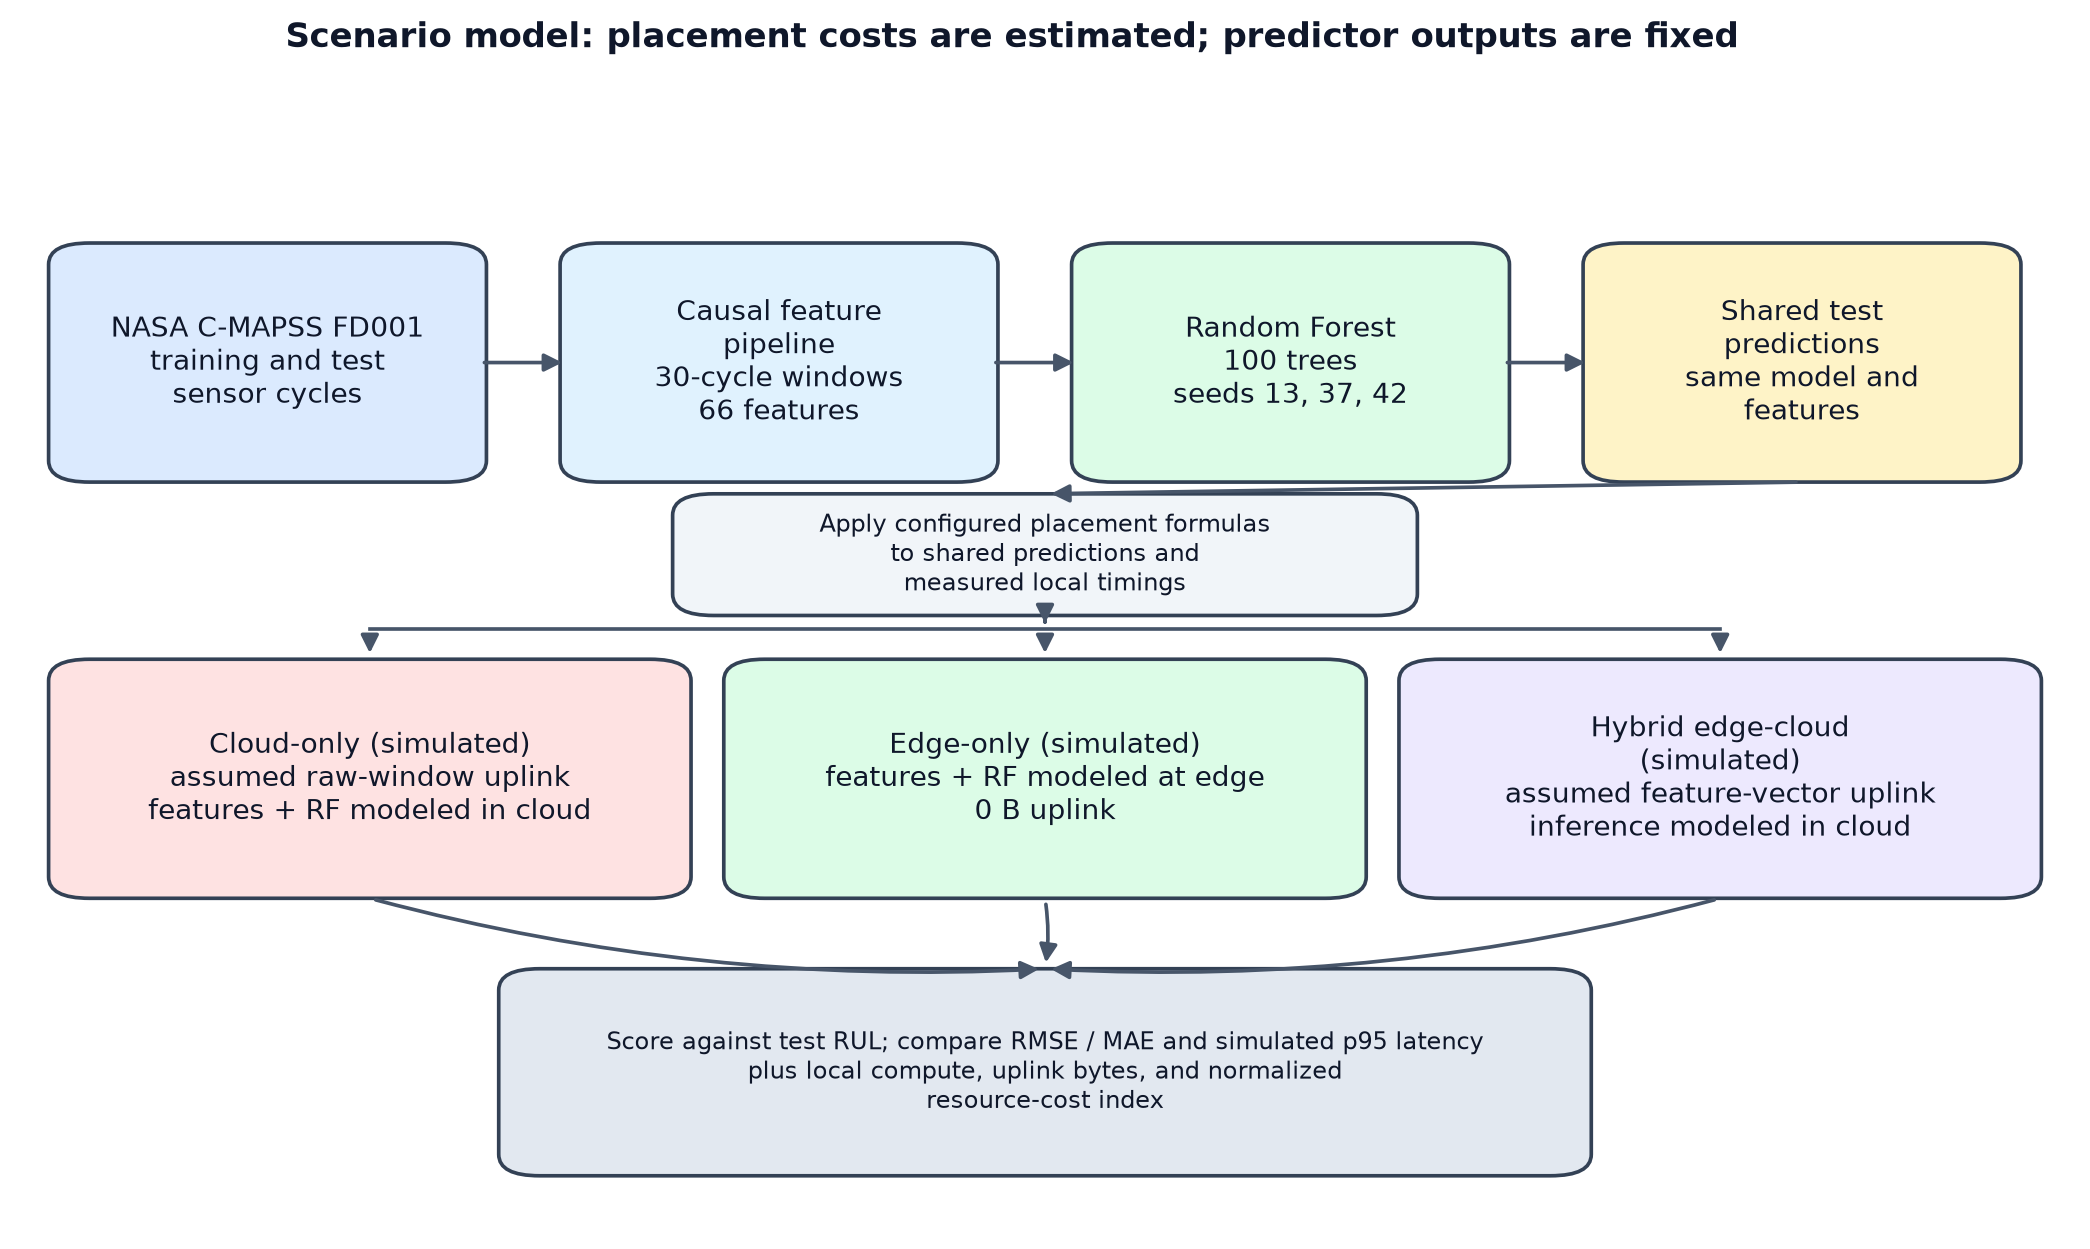
\includegraphics[width=0.98\textwidth]{figures/deployment_architecture.png}
\caption{Implemented experiment workflow and simulated placement scenarios. The simulator reuses fixed predictions and measured local timings; network and edge-compute conditions are configured inputs, not live infrastructure measurements.}
\label{fig:architecture}
\end{figure*}

\subsection{Placement scenarios}
All three scenarios reuse the same prediction vector; the simulator does not perform separate cloud or edge inference. Cloud-only assumes that the 30-cycle, 24-channel window would be sent for remote feature extraction and inference. Edge-only assumes local feature computation and inference with no uplink payload. Hybrid assumes that edge feature extraction precedes remote inference and that the 66-value float32 vector is transmitted. These placements are input/output accounting models, not actual transfers or executions. Accordingly, placement cannot change prediction metrics in this experiment.

Table~\ref{tab:assumptions} lists the scenario parameters. Red bracketed values are explicit assumptions, not empirically measured infrastructure properties. Local feature and model execution times were measured on the experiment workstation: for each request and seed, each function was timed three times and the median duration was used. The scenario model combines those local timings with configured round-trip time (RTT), bandwidth, payload size, and an edge compute multiplier. With feature time $f_i$ and inference time $g_i$ for test engine $i$, the per-request estimates are:
\begin{align}
 L_{\mathrm{cloud},i} &= r_{\mathrm{cloud}}+
 \frac{8b_{\mathrm{raw}}}{1000w}+f_i+g_i,\\
 L_{\mathrm{edge},i} &= r_{\mathrm{edge}}+
 k_{\mathrm{edge}}(f_i+g_i),\\
 L_{\mathrm{hybrid},i} &= r_{\mathrm{cloud}}+
 \frac{8b_{\mathrm{feature}}}{1000w}
 +k_{\mathrm{edge}}f_i+g_i,
\end{align}
where $r$ is RTT in milliseconds, $w$ is bandwidth in Mbps, $b_{\mathrm{raw}}$ and $b_{\mathrm{feature}}$ are assumed payload bytes, and $k_{\mathrm{edge}}$ is the configured edge compute factor. The transfer term converts bits to milliseconds under the configured rate; it assumes no protocol overhead, congestion, packet loss, or competing traffic. The cloud and hybrid scenarios use the same configured RTT, while edge-only uses a smaller configured RTT. These values are not estimates calibrated against named commercial services.

For each scenario, p95 is first calculated across the 100 per-engine latency estimates within a seed, then the table gives the mean and sample standard deviation of those three seed-level p95 values. The reported p95 is therefore not a measured tail latency distribution from a live service. The resource-cost index is a dimensionless, equal-weight proxy,
\begin{equation}
 C=\tfrac{1}{2}\left(\frac{t_{\mathrm{compute}}}{t_{\mathrm{compute,cloud}}}+\frac{b_{\mathrm{uplink}}}{b_{\mathrm{uplink,cloud}}}\right),
\end{equation}
where cloud-only is normalized to one. The index is not a monetary or provider-billing estimate. Requests are evaluated independently; concurrency, queueing, hardware heterogeneity, actual cloud/edge services, network variability, response payloads, and service availability are outside the model.

\begin{table}[t]
\caption{Configured scenario assumptions. Red bracketed values are inputs to the simulator, not measurements.}
\label{tab:assumptions}
\centering
\scriptsize
\setlength{\tabcolsep}{3.5pt}
\begin{tabular}{p{1.4cm}rrp{2.25cm}}
\toprule
\shortstack{Placement} & \shortstack{RTT\\(ms)} & \shortstack{Rate\\(Mbps)} & \shortstack{Compute\\placement} \\
\midrule
Cloud-only & \simval{80} & \simval{20} & Feature extraction and inference modeled in cloud \\
Edge-only & \simval{1} & \simval{20} & Local compute factor \simval{2.0} \\
Hybrid & \simval{80} & \simval{20} & Edge feature factor \simval{2.0}; remote inference \\
\bottomrule
\end{tabular}
\end{table}

\section{Implementation and Experiments}
The workflow has four steps: (1) read the three official FD001 files and record their SHA-256 digests; (2) create causal rolling features and capped training targets; (3) fit the Random Forest and training-mean baseline with each of three seeds, then evaluate once on the same official 100-engine test split; and (4) time local feature/model functions and pass these durations, predictions, and the JSON scenario configuration to the placement simulator. The simulator emits one row per seed and scenario; a separate aggregation step reports mean and sample standard deviation. This sequencing prevents a simulator branch from quietly substituting different predictions or accuracy scores.

The implementation was run on Windows 11 with Python 3.14.6, NumPy 2.5.5, scikit-learn 1.9.1, and Matplotlib 3.11.2 on an AMD64 processor with 12 logical CPUs. The complete run manifest records versions, host information, dataset hashes, estimator settings, seeds, and the deployment configuration digest. The local fit times in the model-run CSV are ordinary workstation measurements and are presented only as such; they are not cloud-versus-edge timing comparisons. Environment changes and CPU scheduling may affect timing results even when the data and model outputs reproduce.

The evaluation is a fixed test-set experiment, not cross-validation. C-MAPSS's official test labels are used only for the final reported metrics. There is no model search against those labels, and no competing deep model is re-trained in this work. Since the three seeds reuse the same training/test data and differ only in Random Forest randomness, they should not be interpreted as three independent datasets or as evidence of population-wide uncertainty.

For descriptive error analysis, we also aggregate engine-level metrics into four test-label intervals: 0--30, 31--60, 61--90, and greater than 90 cycles. The bins are based on official final-cycle RUL labels after prediction; they are not used in training, feature construction, or model selection. The supplementary analysis script repeats the same three seeds, evaluates the same test predictions against each bin, and writes per-seed and summary CSVs. This reports heterogeneity in the fixed test set, not performance on new cohorts.

\section{Results}
\subsection{Measured prediction results}
Table~\ref{tab:seedresults} reports the actual test metrics and local fit time from each run. Across seeds, the Random Forest obtains RMSE $15.0266\pm0.5049$ cycles and MAE $11.8558\pm0.4167$ cycles. The constant training-mean baseline obtains RMSE 43.0670 and MAE 35.9000 in all three runs. Relative to this baseline, the RF reduces mean RMSE by 65.1\% and mean MAE by 67.0\%, calculated from the raw metrics. This establishes that the implemented features carry predictive signal against a constant estimate on this official split, but the weak baseline does not establish competitiveness with specialized prognostic methods.

The RF RMSE ranges from 14.6943 to 15.6076 across seeds, and MAE ranges from 11.5254 to 12.3240. These variations are meaningful to report because the test set contains only 100 engines, but the runs are repeated fits on the same examples, not independent test samples. The mean fit time is 4.755 s (sample SD 0.159 s) on the recorded workstation. Fit time is a local observation and is not used as a cloud or edge latency result.

\begin{table*}[t]
\caption{Actual FD001 test-set metrics and local Random Forest fit time by seed. Values are from the experiment output files.}
\label{tab:seedresults}
\centering
\scriptsize
\setlength{\tabcolsep}{3.5pt}
\begin{tabular}{crrrr r}
\toprule
Seed & \shortstack{RF RMSE\\(cycles)} & \shortstack{RF MAE\\(cycles)} & \shortstack{RF fit\\time (s)} & \shortstack{Mean RMSE\\(cycles)} & \shortstack{Mean MAE\\(cycles)} \\
\midrule
13 & 14.7780 & 11.7181 & 4.672 & 43.0670 & 35.9000 \\
37 & 14.6943 & 11.5254 & 4.938 & 43.0670 & 35.9000 \\
42 & 15.6076 & 12.3240 & 4.654 & 43.0670 & 35.9000 \\
\midrule
Mean $\pm$ sample SD & $15.0266\pm0.5049$ & $11.8558\pm0.4167$ & $4.755\pm0.159$ & $43.0670\pm0.0000$ & $35.9000\pm0.0000$ \\
\bottomrule
\end{tabular}
\end{table*}

\subsection{Measured error by official RUL range}
Table~\ref{tab:rulrange} gives a second view of actual test performance. In the 0--30, 31--60, and $>90$ cycle groups, the RF's mean MAE is lower than the training-mean baseline. The 61--90 group is an exception: on 15 engines, the baseline MAE is 8.12 cycles versus 21.96 for the RF. This descriptive result shows that aggregate scores hide target-range variation; it does not establish a general advantage for the constant baseline in this range, because subgroup sizes are small and all engines come from the same benchmark condition.

\begin{table*}[t]
\caption{Actual FD001 test errors stratified by official final-cycle RUL. RF values are mean $\pm$ sample SD over three seeds; baseline values are unchanged across seeds.}
\label{tab:rulrange}
\centering
\scriptsize
\setlength{\tabcolsep}{3pt}
\begin{tabular}{lrrrrr}
\toprule
True RUL (cycles) & Engines & RF RMSE & RF MAE & Mean RMSE & Mean MAE \\
\midrule
0--30 & 25 & $8.20\pm0.49$ & $5.51\pm0.30$ & 69.49 & 69.11 \\
31--60 & 14 & $13.20\pm0.78$ & $10.73\pm0.57$ & 37.97 & 37.12 \\
61--90 & 15 & $23.29\pm1.17$ & $21.96\pm1.23$ & 10.94 & 8.12 \\
$>90$ & 46 & $14.97\pm0.19$ & $12.35\pm0.19$ & 30.49 & 26.54 \\
\bottomrule
\end{tabular}
\end{table*}

\subsection{Simulated placement outcomes}
Table~\ref{tab:results} keeps the measured accuracy columns in black and brackets all scenario-derived quantities in red. The three rows contain identical RMSE and MAE by construction: they use each seed's same trained model and predictions. Scenario p95, compute, payload, and cost are estimates from the formulas and assumptions, not empirically observed deployments. For hybrid, the assumed feature payload is \simval{264} bytes rather than the cloud-only raw-window payload of \simval{2880} bytes; the resulting percentage is a calculation from these modeled byte counts.

\begin{table*}[t]
\caption{Actual FD001 prediction results and simulator-derived placement estimates. Black values are measured test metrics; red bracketed values are assumption-derived outputs.}
\label{tab:results}
\centering
\scriptsize
\setlength{\tabcolsep}{4pt}
\begin{tabular}{lrrrrrr}
\toprule
Scenario & RMSE (cycles) & MAE (cycles) & p95 (ms) & Compute (ms) & Uplink (bytes) & Cost index \\
\midrule
Cloud-only & $15.0266\pm0.5049$ & $11.8558\pm0.4167$ & \simval{$111.322\pm0.422$} & \simval{28.478} & \simval{2880} & \simval{1.000} \\
Edge-only & $15.0266\pm0.5049$ & $11.8558\pm0.4167$ & \simval{$61.339\pm0.844$} & \simval{56.955} & \simval{0} & \simval{1.000} \\
Hybrid edge--cloud & $15.0266\pm0.5049$ & $11.8558\pm0.4167$ & \simval{$110.326\pm0.405$} & \simval{28.521} & \simval{264} & \simval{0.547} \\
\bottomrule
\end{tabular}
\end{table*}

The estimated edge-only p95 is \simval{61.339} ms versus \simval{111.322} ms for cloud-only, a scenario-model reduction of about \simval{44.9\%}; this follows primarily from the configured RTT difference and does not demonstrate a faster deployed system. The hybrid scenario retains the configured cloud RTT and estimates p95 of \simval{110.326} ms. Its assumed input payload reduction from \simval{2880} to \simval{264} bytes equals \simval{90.83\%}. The normalized cost proxy for hybrid is \simval{0.547}, while the edge-only index equals \simval{1.000} because the formula balances a doubled compute ratio against zero modeled uplink. None of these bracketed comparisons should be interpreted as measured service performance, actual network traffic, or monetary savings.

Fig.~\ref{fig:tradeoffs} shows the generated deployment-tradeoff figure. Its latency and resource comparisons inherit the same simulation assumptions and do not establish real-world service-level performance.
\begin{figure}[t]
\centering
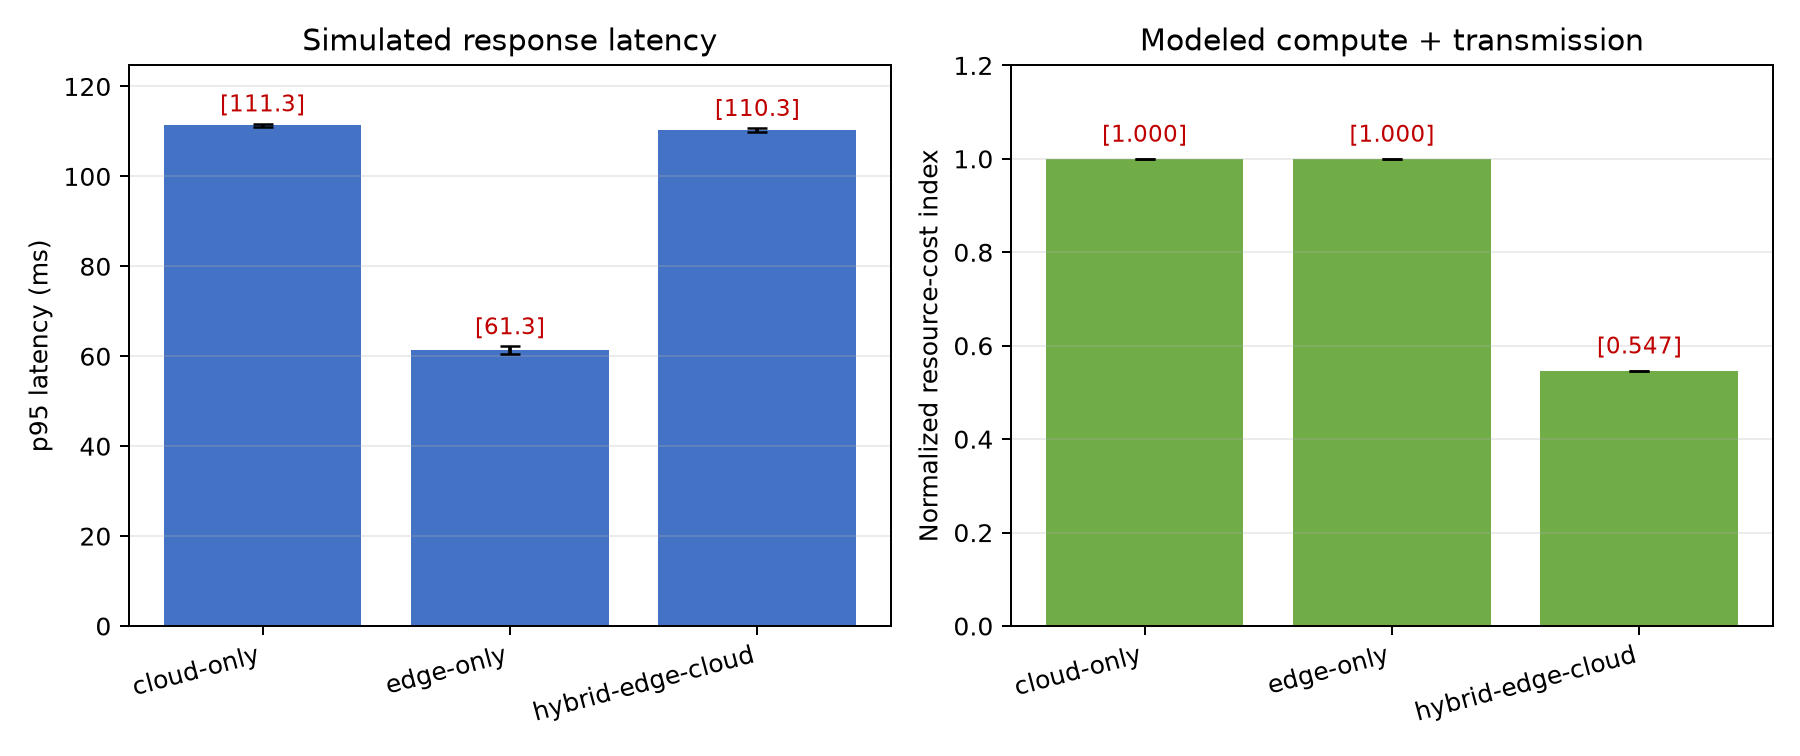
\includegraphics[width=\columnwidth]{figures/deployment_tradeoffs.png}
\caption{Scenario-derived p95 latency and normalized cost proxy. Red bracketed labels are estimates from the configured simulator, not measurements from a cloud or edge service. Accuracy is measured and shared across scenarios.}
\label{fig:tradeoffs}
\end{figure}

\section{Discussion}
The experiment separates model quality from scenario arithmetic. The only measured accuracy values come from the RF and mean baseline on the official FD001 test set; their placement rows repeat because each scenario uses the same prediction vector. The RF's 65.1\% RMSE and 67.0\% MAE reductions against the training-mean estimate are actual benchmark outcomes from this pipeline and split. They are not evidence of improvement over the deep-learning methods cited in Related Work, because those methods and this study do not share an experimentally controlled pipeline and evaluation protocol.

The scenario exercise is useful as a sensitivity illustration. Under the declared constants, cloud and hybrid include the same nominal wide-area RTT while edge-only has a smaller nominal RTT; consequently, edge-only is the fastest simulated branch even though its compute component is multiplied by two. Hybrid lowers the assumed uplink payload while retaining remote inference, so it remains close to cloud-only in estimated latency. These outcomes are largely determined by the selected constants. Changing RTT, bandwidth, transfer overhead, or the compute factor could change the ordering; readers can edit the JSON file and rerun the analysis to inspect such alternatives. The equal-weight cost index is likewise a modeling choice, not a validated utility function.

The scenario comparison also exposes what this code does not test. No physical asset state is streamed, no actual edge device extracts features, no remote server receives the hybrid payload, and no service-level latency distribution is collected. Local function timing is reused in a formula; calling that value an edge or cloud benchmark would be incorrect. Therefore the manuscript labels scenario values in red brackets and reports the measured prediction metrics separately. This separation is a core reproducibility feature, not a cosmetic convention.

For practitioners, the most defensible conclusion is procedural: assess prognostic accuracy and infrastructure behavior as separate measurements, and report assumptions whenever using simulation to compare placements. A future study with the same model on specified hardware could measure serialized payloads, end-to-end RTT, edge power, memory, and request concurrency. Only then could one test whether these modeled tendencies transfer to an operational PdM deployment.

\section{Limitations and Threats to Validity}
\subsection{Dataset and construct validity}
The dataset scope is limited to FD001, with 20,631 generated training windows and only 100 test engines. FD001 represents a single operating condition and fault mode; results do not establish generalization to FD002--FD004, other assets, or field telemetry. The benchmark supplies simulated degradation trajectories and RUL labels, not observed maintenance interventions, economic costs, or a fleet operator's failure criterion. Consequently, RMSE and MAE quantify prediction error in cycles only; they do not measure avoided downtime, safety, or maintenance utility.

The fixed 30-cycle summary features discard temporal detail beyond three statistics per sensor. Their simplicity makes the transformation inspectable, but may suppress phase-specific dynamics. The training-label cap at 125 cycles also changes the target distribution, while test labels remain official and uncapped. The reported aggregate scores should therefore be interpreted with the subgroup table and the exact label policy, not as a universal accuracy number.

\subsection{Model and statistical validity}
The RF hyperparameters and baseline are fixed, and the intentionally weak training-mean predictor is not a strong literature baseline. We do not reimplement or tune a neural method from the related-work set under an identical split. Thus the results support only the claim that this implementation outperforms a constant training-mean prediction overall on this test set; they do not establish state-of-the-art performance. The 61--90-cycle subgroup further shows why aggregate improvements alone can hide a range where the baseline is better.

Three seeds capture variability due to Random Forest randomness while holding data fixed. They do not provide independent samples of engines or operating conditions, and their standard deviations are not confidence intervals. The RUL-bin analysis is descriptive and uses test labels only to report errors after prediction; it must not be used to select deployment settings or hyperparameters. A larger evaluation should include repeated engine-level protocols, additional subsets, and external data.

\subsection{Deployment-model validity}
No cloud or edge service was deployed. Fixed RTT, bandwidth, and compute-factor assumptions are scenario inputs rather than empirical measurements, and the simulator excludes serialization overhead, protocol behavior, congestion, queueing, concurrent requests, hardware-specific power, and service billing. Locally timed feature and inference functions are reused as formula inputs; those times are not equivalent to cloud or edge measurements. The equal-weight compute/byte index has no calibrated economic interpretation. Accordingly, all derived deployment values remain red-bracketed and must not be read as observed infrastructure performance.

\subsection{Digital-twin scope}
The implementation does not maintain a persistent synchronized asset state, ingest live sensor streams, trigger fault alerts, recommend maintenance actions, or close the loop using post-maintenance observations. It evaluates a prognostic model and a set of placement calculations that could inform one component of a future twin. The work is therefore a reproducible PdM software experiment in a digital-twin context, not a complete or deployed digital-twin system.

\section{Conclusion}
A single FD001 Random Forest baseline produced measured mean RMSE $15.0266\pm0.5049$ and MAE $11.8558\pm0.4167$ cycles across three seeds, respectively 65.1\% and 67.0\% lower than the training-mean baseline on this test split. Under the declared assumptions, the estimated edge-only p95 is \simval{61.339} ms and hybrid modeled uplink is \simval{90.83\%} lower than cloud-only; these red-bracketed outputs are not physical measurements. The paper's central result is thus twofold: it provides actual, reproducible benchmark accuracy for the implemented pipeline and an auditable but simulated comparison of placement formulas. Future work should evaluate all four C-MAPSS subsets, compare additional prognostic models under matched protocols, and measure serialized traffic, end-to-end latency, power, and cost on specified physical edge and cloud services before making operational claims.

\section*{Reproducibility}
The public repository contains the implementation, pinned Python requirements, deployment JSON, raw per-seed result CSVs, aggregate tables, figure generators, and run manifest with SHA-256 digests for the three official FD001 input files. After placing the official files in \texttt{data/raw/}, the main workflow is reproduced from the repository root with \texttt{python -m src.data\_prep}, followed by \texttt{python -m experiments.run\_all}. The additional actual error-by-RUL-range analysis is generated with \texttt{python -m experiments.rul\_range\_analysis}; it writes one per-seed CSV and one mean/sample-standard-deviation summary. Figures are regenerated with \texttt{python -m src.plot\_results} and \texttt{python -m src.plot\_architecture}. The raw NASA files are not redistributed in the repository; the README identifies the archive and extraction paths.

Code, configurations, results, and reproduction instructions are available at \url{https://github.com/m-ayan-asif/ai-driven-digital-twins-for-predictive-maintenance}.

\begin{thebibliography}{32}
\bibitem{tao2018} F. Tao, M. Zhang, Y. Liu, and A. Y. C. Nee, ``Digital twin driven prognostics and health management for complex equipment,'' \emph{CIRP Annals}, vol. 67, no. 1, pp. 169--172, 2018, doi: 10.1016/j.cirp.2018.04.055.
\bibitem{toothman2023} M. Toothman, B. Braun, S. J. Bury, J. Moyne, D. M. Tilbury, Y. Ye, and K. Barton, ``A digital twin framework for prognostics and health management,'' \emph{Computers in Industry}, vol. 150, Art. no. 103948, 2023, doi: 10.1016/j.compind.2023.103948.
\bibitem{asif2022} O. Asif, S. A. Haider, S. R. Naqvi, J. F. W. Zaki, K.-S. Kwak, and S. M. R. Islam, ``A deep learning model for remaining useful life prediction of aircraft turbofan engine on C-MAPSS dataset,'' \emph{IEEE Access}, vol. 10, pp. 95425--95440, 2022, doi: 10.1109/ACCESS.2022.3203406.
\bibitem{aldulaimi2019} A. Al-Dulaimi, S. Zabihi, A. Asif, and A. Mohammadi, ``A multimodal and hybrid deep neural network model for remaining useful life estimation,'' \emph{Computers in Industry}, vol. 108, pp. 186--196, 2019, doi: 10.1016/j.compind.2019.02.004.
\bibitem{firouzi2022} F. Firouzi, B. Farahani, and A. Marin\v{s}ek, ``The convergence and interplay of edge, fog, and cloud in the AI-driven Internet of Things (IoT),'' \emph{Information Systems}, vol. 107, Art. no. 101840, 2022, doi: 10.1016/j.is.2021.101840.
\bibitem{shi2016} W. Shi, J. Cao, Q. Zhang, Y. Li, and L. Xu, ``Edge computing: Vision and challenges,'' \emph{IEEE Internet of Things Journal}, vol. 3, no. 5, pp. 637--646, 2016, doi: 10.1109/JIOT.2016.2579198.
\bibitem{fuller2020} A. Fuller, Z. Fan, C. Day, and C. Barlow, ``Digital twin: Enabling technologies, challenges and open research,'' \emph{IEEE Access}, vol. 8, pp. 108952--108971, 2020, doi: 10.1109/ACCESS.2020.2998358.
\bibitem{tao2019} F. Tao, H. Zhang, A. Liu, and A. Y. C. Nee, ``Digital twin in industry: State-of-the-art,'' \emph{IEEE Transactions on Industrial Informatics}, vol. 15, no. 4, pp. 2405--2415, 2019, doi: 10.1109/TII.2018.2873186.
\bibitem{rasheed2020} A. Rasheed, O. San, and T. Kvamsdal, ``Digital twin: Values, challenges and enablers from a modeling perspective,'' \emph{IEEE Access}, vol. 8, pp. 21980--22012, 2020, doi: 10.1109/ACCESS.2020.2970143.
\bibitem{barricelli2019} B. R. Barricelli, E. Casiraghi, and D. Fogli, ``A survey on digital twin: Definitions, characteristics, applications, and design implications,'' \emph{IEEE Access}, vol. 7, pp. 167653--167671, 2019, doi: 10.1109/ACCESS.2019.2953499.
\bibitem{jones2020} M. Jones, C. Snider, A. Nassehi, J. Yon, and B. Hicks, ``Characterising the digital twin: A systematic literature review,'' \emph{CIRP Journal of Manufacturing Science and Technology}, vol. 29, pp. 36--52, 2020, doi: 10.1016/j.cirpj.2020.02.002.
\bibitem{semeraro2021} R. Semeraro, N. Lezoche, H. Panetto, and M. Dassisti, ``Digital twin paradigm: A systematic literature review,'' \emph{Computers in Industry}, vol. 130, Art. no. 103469, 2021, doi: 10.1016/j.compind.2021.103469.
\bibitem{cimino2019} C. Cimino, E. Negri, and L. Fumagalli, ``Review of digital twin applications in manufacturing,'' \emph{Computers in Industry}, vol. 113, Art. no. 103130, 2019, doi: 10.1016/j.compind.2019.103130.
\bibitem{jardine2006} A. K. S. Jardine, D. Lin, and D. Banjevic, ``A review on machinery diagnostics and prognostics implementing condition-based maintenance,'' \emph{Mechanical Systems and Signal Processing}, vol. 20, no. 7, pp. 1483--1510, 2006, doi: 10.1016/j.ymssp.2005.09.012.
\bibitem{si2011} X. Si, W. Wang, C. Hu, and D.-H. Zhou, ``Remaining useful life estimation: A review on the statistical data driven approaches,'' \emph{European Journal of Operational Research}, vol. 213, no. 1, pp. 1--14, 2011, doi: 10.1016/j.ejor.2010.11.018.
\bibitem{peng2010} Y. Peng, M. Dong, and M. J. Zuo, ``Current status of machine prognostics in condition-based maintenance: A review,'' \emph{The International Journal of Advanced Manufacturing Technology}, vol. 50, nos. 1--4, pp. 297--313, 2010, doi: 10.1007/s00170-009-2482-0.
\bibitem{lei2018} Y. Lei, N. Li, L. Guo, N. Li, T. Yan, and J. Lin, ``Machinery health prognostics: A systematic review from data acquisition to RUL prediction,'' \emph{Mechanical Systems and Signal Processing}, vol. 104, pp. 799--834, 2018, doi: 10.1016/j.ymssp.2017.11.016.
\bibitem{carvalho2019} T. P. Carvalho, F. A. A. M. N. Soares, R. Vita, R. da P. Francisco, J. P. Basto, and S. G. S. Alcal\'a, ``A systematic literature review of machine learning methods applied to predictive maintenance,'' \emph{Computers \& Industrial Engineering}, vol. 137, Art. no. 106024, 2019, doi: 10.1016/j.cie.2019.106024.
\bibitem{zonta2020} T. Zonta, C. A. da Costa, R. da Rosa Righi, M. J. de Lima, E. S. da Trindade, and G. Li, ``Predictive maintenance in the Industry 4.0: A systematic literature review,'' \emph{Computers \& Industrial Engineering}, vol. 150, Art. no. 106889, 2020, doi: 10.1016/j.cie.2020.106889.
\bibitem{dalzochio2020} J. Dalzochio et al., ``Machine learning and reasoning for predictive maintenance in Industry 4.0: Current status and challenges,'' \emph{Computers in Industry}, vol. 123, Art. no. 103298, 2020, doi: 10.1016/j.compind.2020.103298.
\bibitem{ahmadzadeh2014} F. Ahmadzadeh and J. Lundberg, ``Remaining useful life estimation: Review,'' \emph{International Journal of System Assurance Engineering and Management}, vol. 5, no. 4, pp. 461--474, 2014, doi: 10.1007/s13198-013-0195-0.
\bibitem{xue2022} B. Xue, H. Xu, X. Huang, K. Zhu, Z. Xu, and H. Pei, ``Similarity-based prediction method for machinery remaining useful life: A review,'' \emph{The International Journal of Advanced Manufacturing Technology}, vol. 121, nos. 3--4, pp. 1501--1531, 2022, doi: 10.1007/s00170-022-09280-3.
\bibitem{zhang2023} Y. Zhang, L. Fang, Z. Qi, and H. Deng, ``A review of remaining useful life prediction approaches for mechanical equipment,'' \emph{IEEE Sensors Journal}, vol. 23, no. 24, pp. 29991--30006, 2023, doi: 10.1109/JSEN.2023.3326487.
\bibitem{ellefsen2019} A. L. Ellefsen et al., ``Remaining useful life predictions for turbofan engine degradation using semi-supervised deep architecture,'' \emph{Reliability Engineering \& System Safety}, vol. 183, pp. 240--251, 2019, doi: 10.1016/j.ress.2018.11.027.
\bibitem{zhao2019} R. Zhao, R. Yan, Z. Chen, K. Mao, P. Wang, and R. X. Gao, ``Deep learning and its applications to machine health monitoring,'' \emph{Mechanical Systems and Signal Processing}, vol. 115, pp. 213--237, 2019, doi: 10.1016/j.ymssp.2018.05.050.
\bibitem{li2023} J. Li, Y. Jia, M. Niu, W. Zhu, and F. Meng, ``Remaining useful life prediction of turbofan engines using CNN-LSTM-SAM approach,'' \emph{IEEE Sensors Journal}, vol. 23, no. 9, pp. 10241--10251, 2023, doi: 10.1109/JSEN.2023.3261874.
\bibitem{mao2017} Y. Mao, C. You, J. Zhang, K. Huang, and K. B. Letaief, ``A survey on mobile edge computing: The communication perspective,'' \emph{IEEE Communications Surveys \& Tutorials}, vol. 19, no. 4, pp. 2322--2358, 2017, doi: 10.1109/COMST.2017.2745201.
\bibitem{abbas2018} N. Abbas, Y. Zhang, A. Taherkordi, and T. Skeie, ``Mobile edge computing: A survey,'' \emph{IEEE Internet of Things Journal}, vol. 5, no. 1, pp. 450--465, 2018, doi: 10.1109/JIOT.2017.2750180.
\bibitem{zhou2019} Z. Zhou et al., ``Edge intelligence: Paving the last mile of artificial intelligence with edge computing,'' \emph{Proceedings of the IEEE}, vol. 107, no. 8, pp. 1738--1762, 2019, doi: 10.1109/JPROC.2019.2918951.
\bibitem{satya2017} M. Satyanarayanan, ``The emergence of edge computing,'' \emph{Computer}, vol. 50, no. 1, pp. 30--39, 2017, doi: 10.1109/MC.2017.9.
\bibitem{chiang2016} M. Chiang and T. Zhang, ``Fog and IoT: An overview of research opportunities,'' \emph{IEEE Internet of Things Journal}, vol. 3, no. 6, pp. 854--864, 2016, doi: 10.1109/JIOT.2016.2584538.
\bibitem{naha2018} R. K. Naha et al., ``Fog computing: Survey of trends, architectures, requirements, and research directions,'' \emph{IEEE Access}, vol. 6, pp. 47980--48009, 2018, doi: 10.1109/ACCESS.2018.2866491.
\end{thebibliography}

\end{document}
